\section{2.7}

Problem description:
\begin{figure} [H]
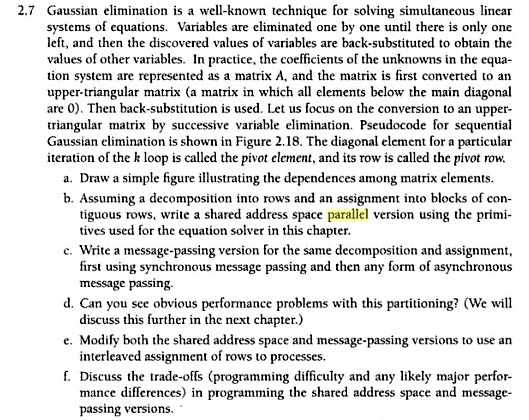
\includegraphics[width=\textwidth]{figures/2-7-problem.jpg}
\end{figure}

\begin{figure} [H]
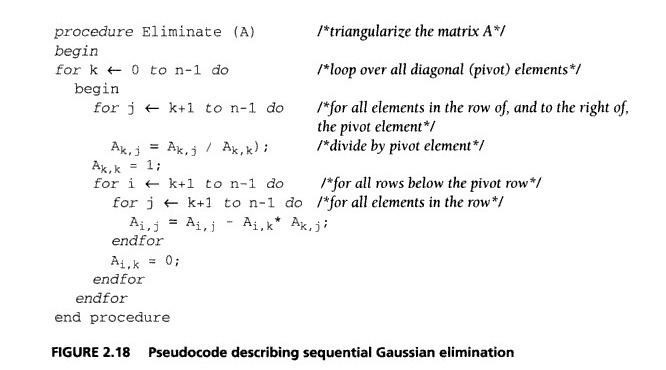
\includegraphics[width=\textwidth]{figures/figure2-18.jpg}
\caption{figure 2.18}
\end{figure} 

\subsection{2.7(a)}

There are three cases as showed following. Red is used to mark the target entry. 
Shadow area shows the dependent entries in the matrix. 

\begin{figure} [H]
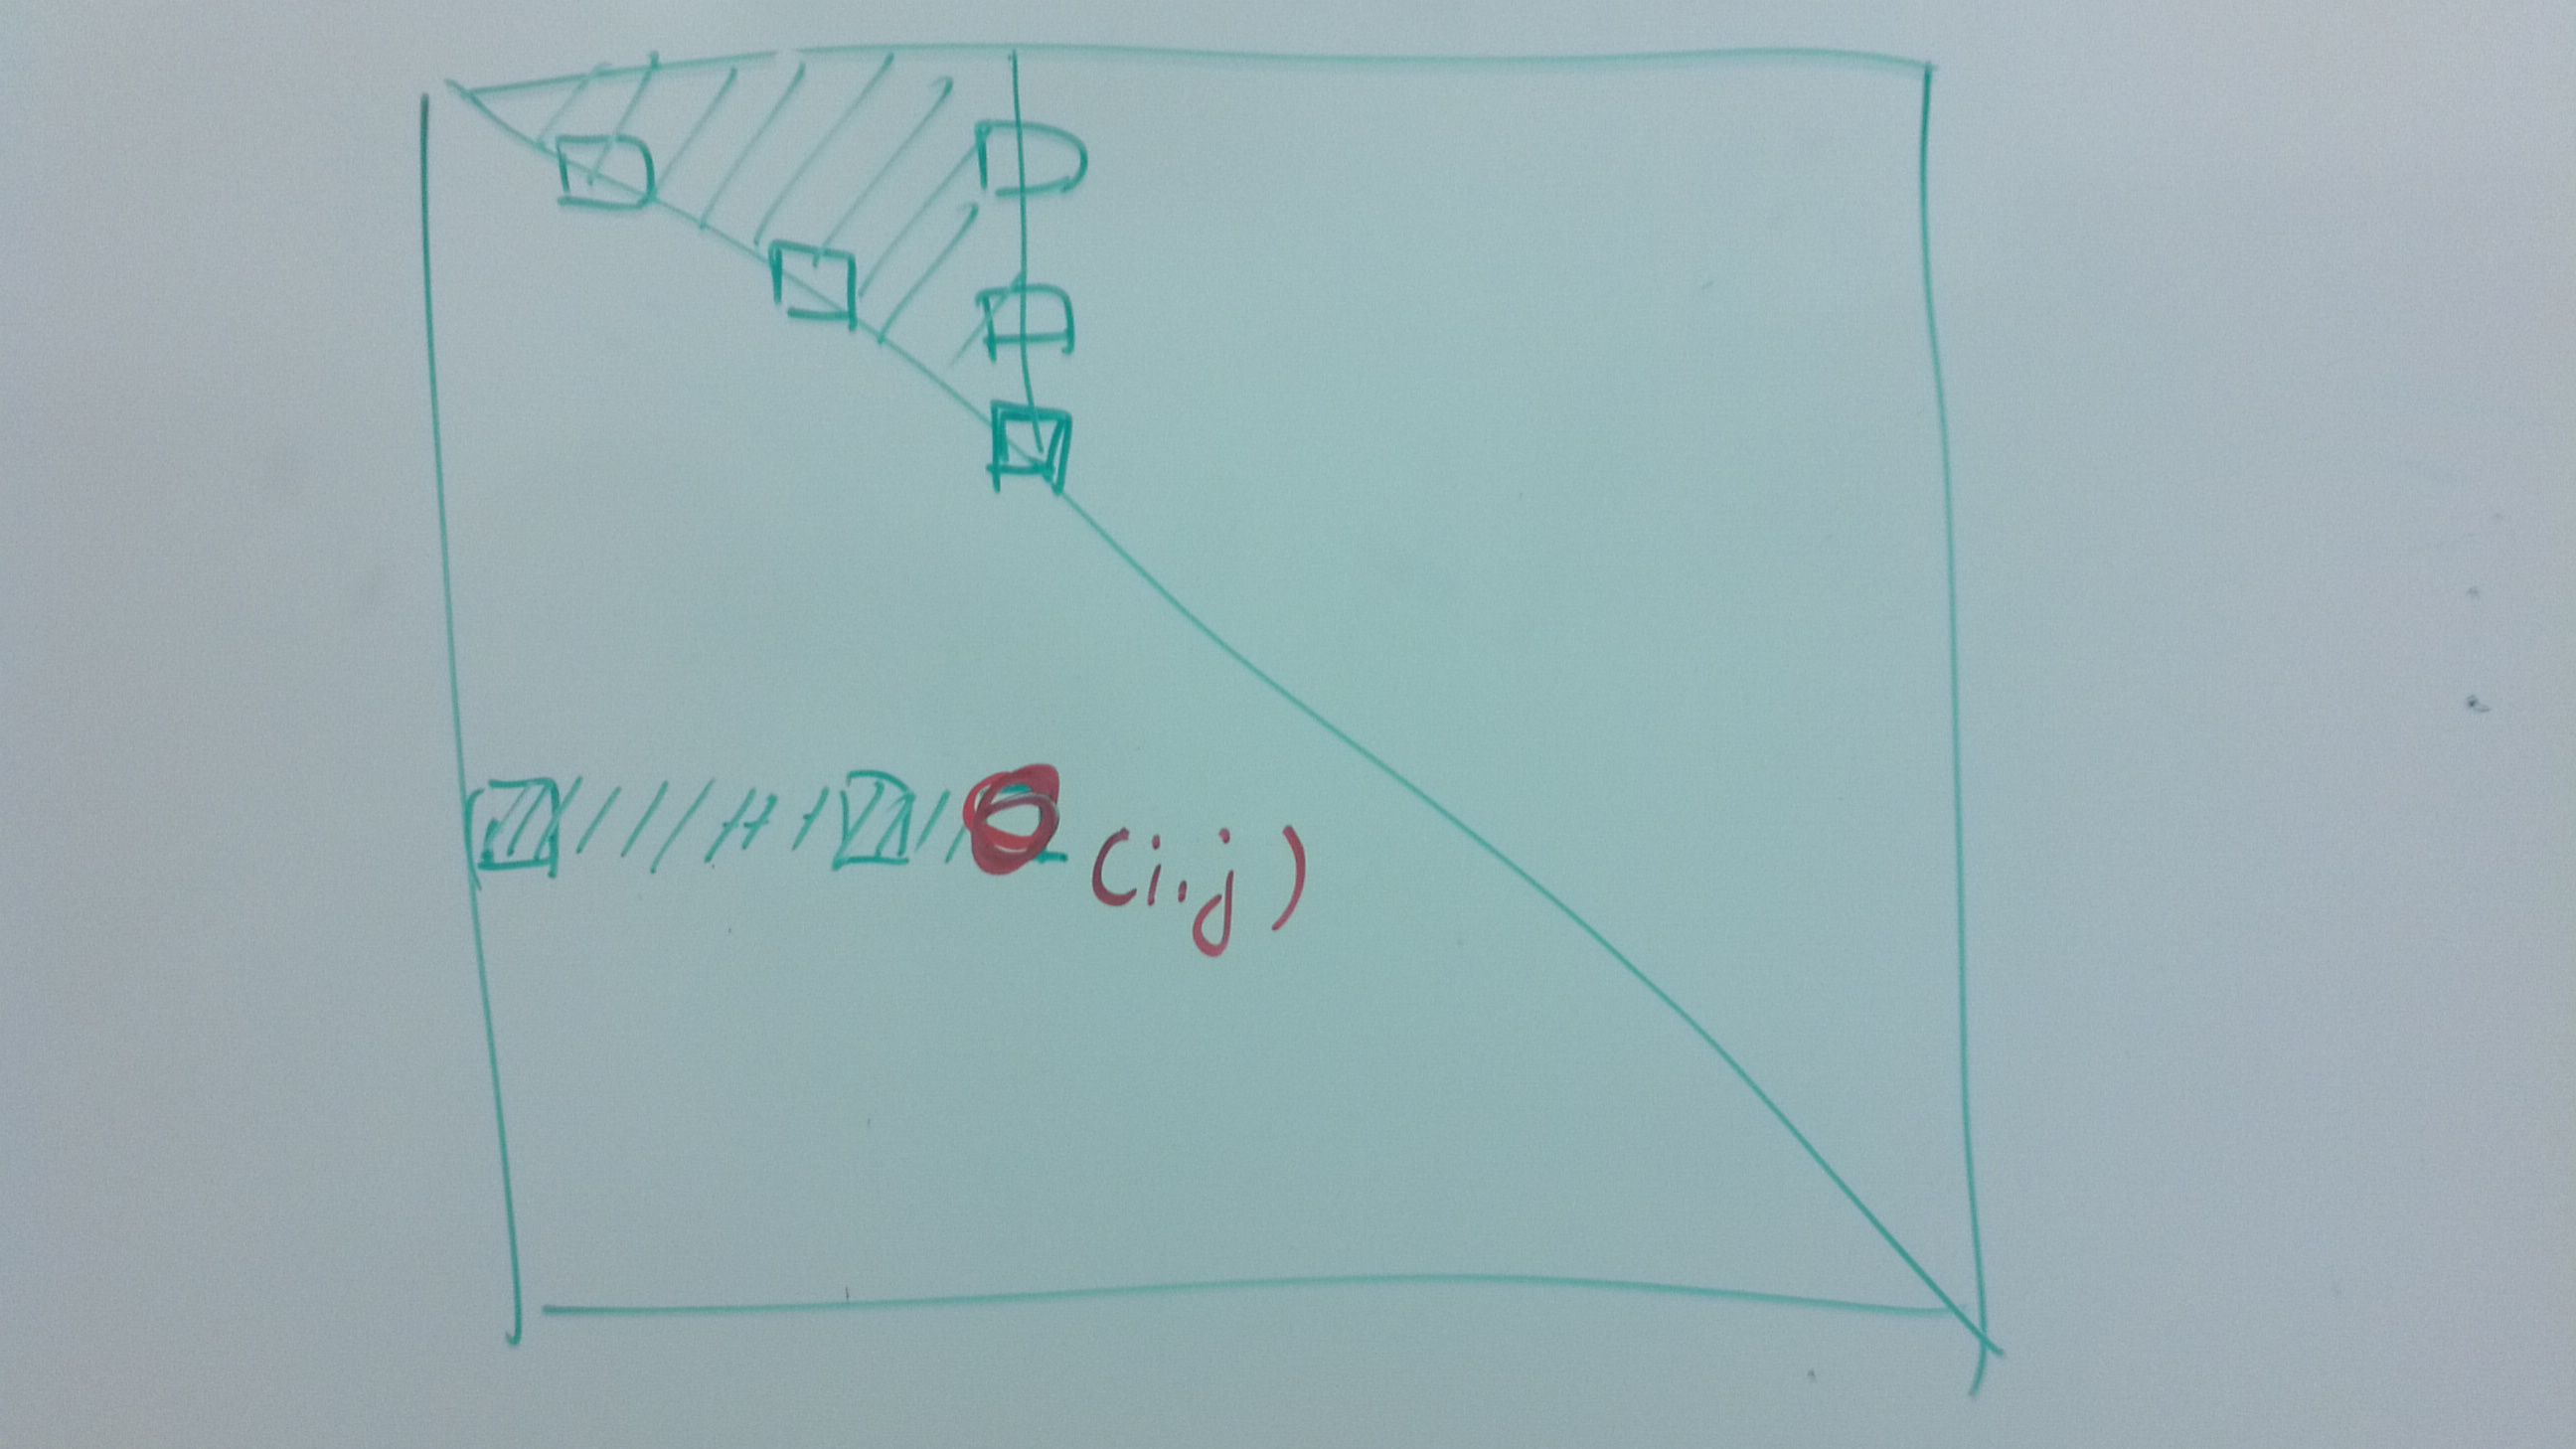
\includegraphics[width=\textwidth]{figures/a1.jpg}
\caption{dependences of entry $a_{i,j}$, where i > j}
\end{figure}

\begin{figure} [H]
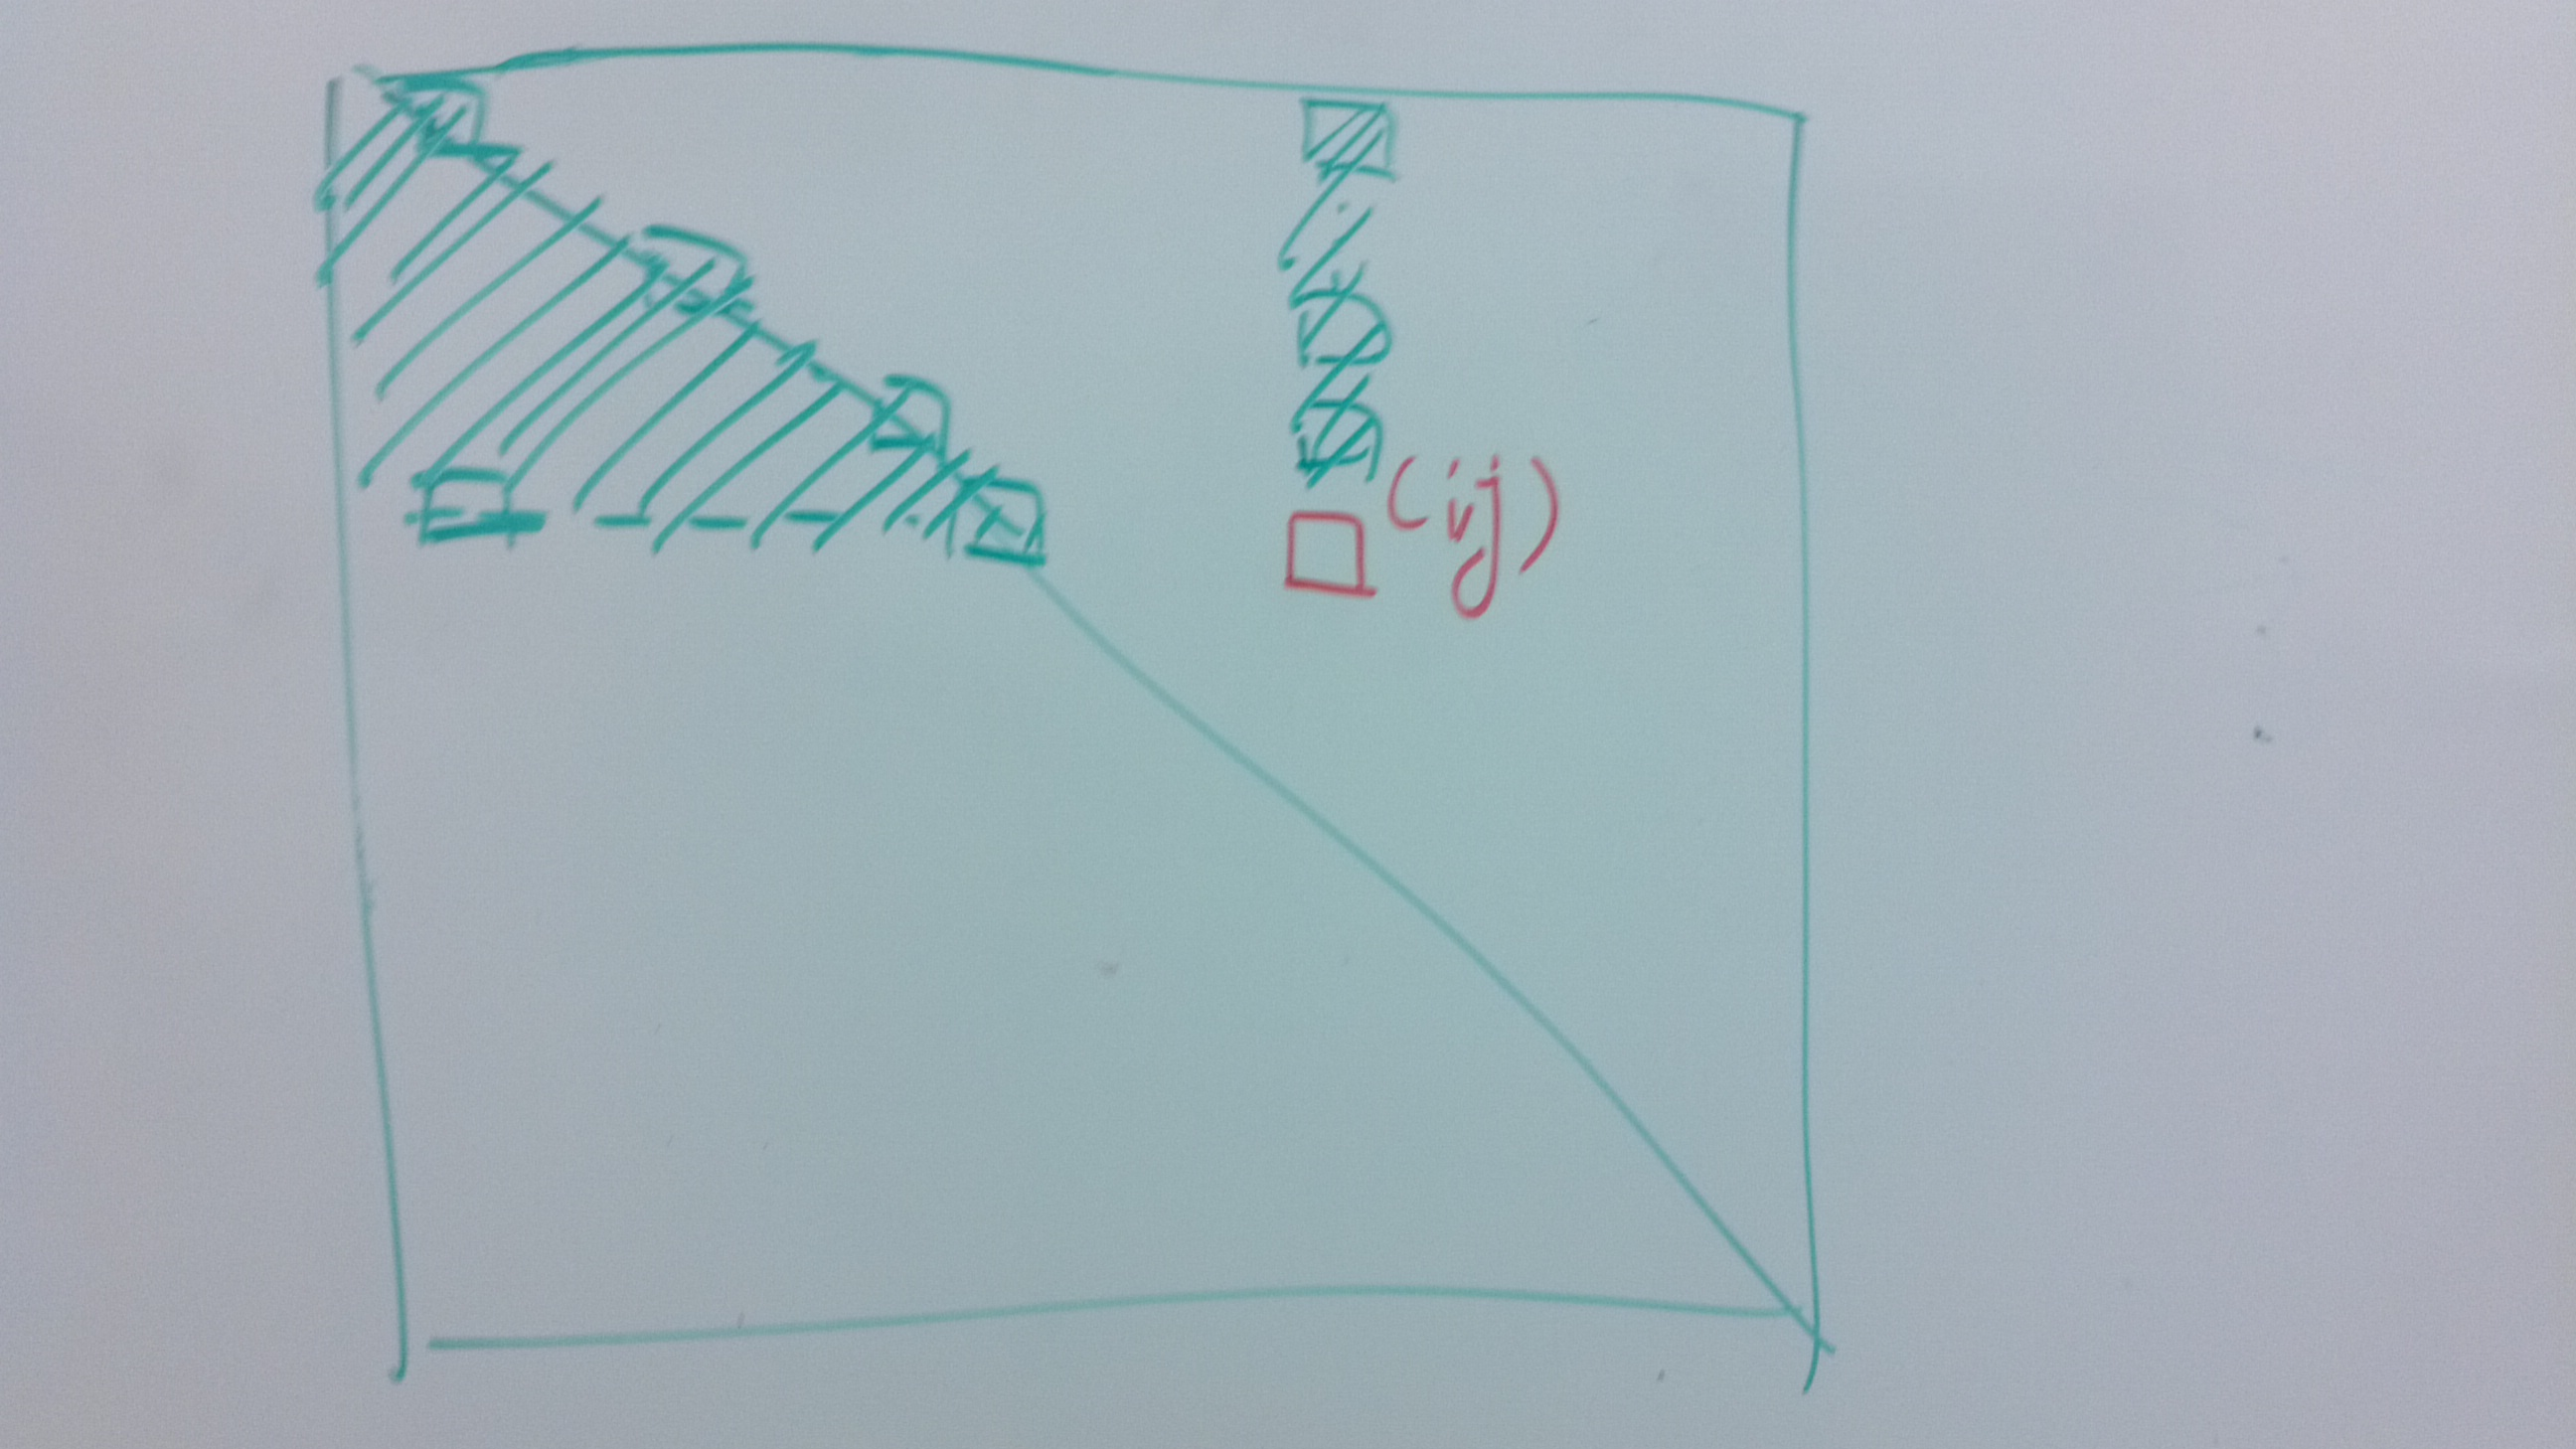
\includegraphics[width=\textwidth]{figures/a2.jpg}
\caption{dependences of entry $a_{i,j}$, where i < j}
\end{figure}

In the last case, we have $a_{i,j}$ for $i = j$. 
\begin{figure} [H]
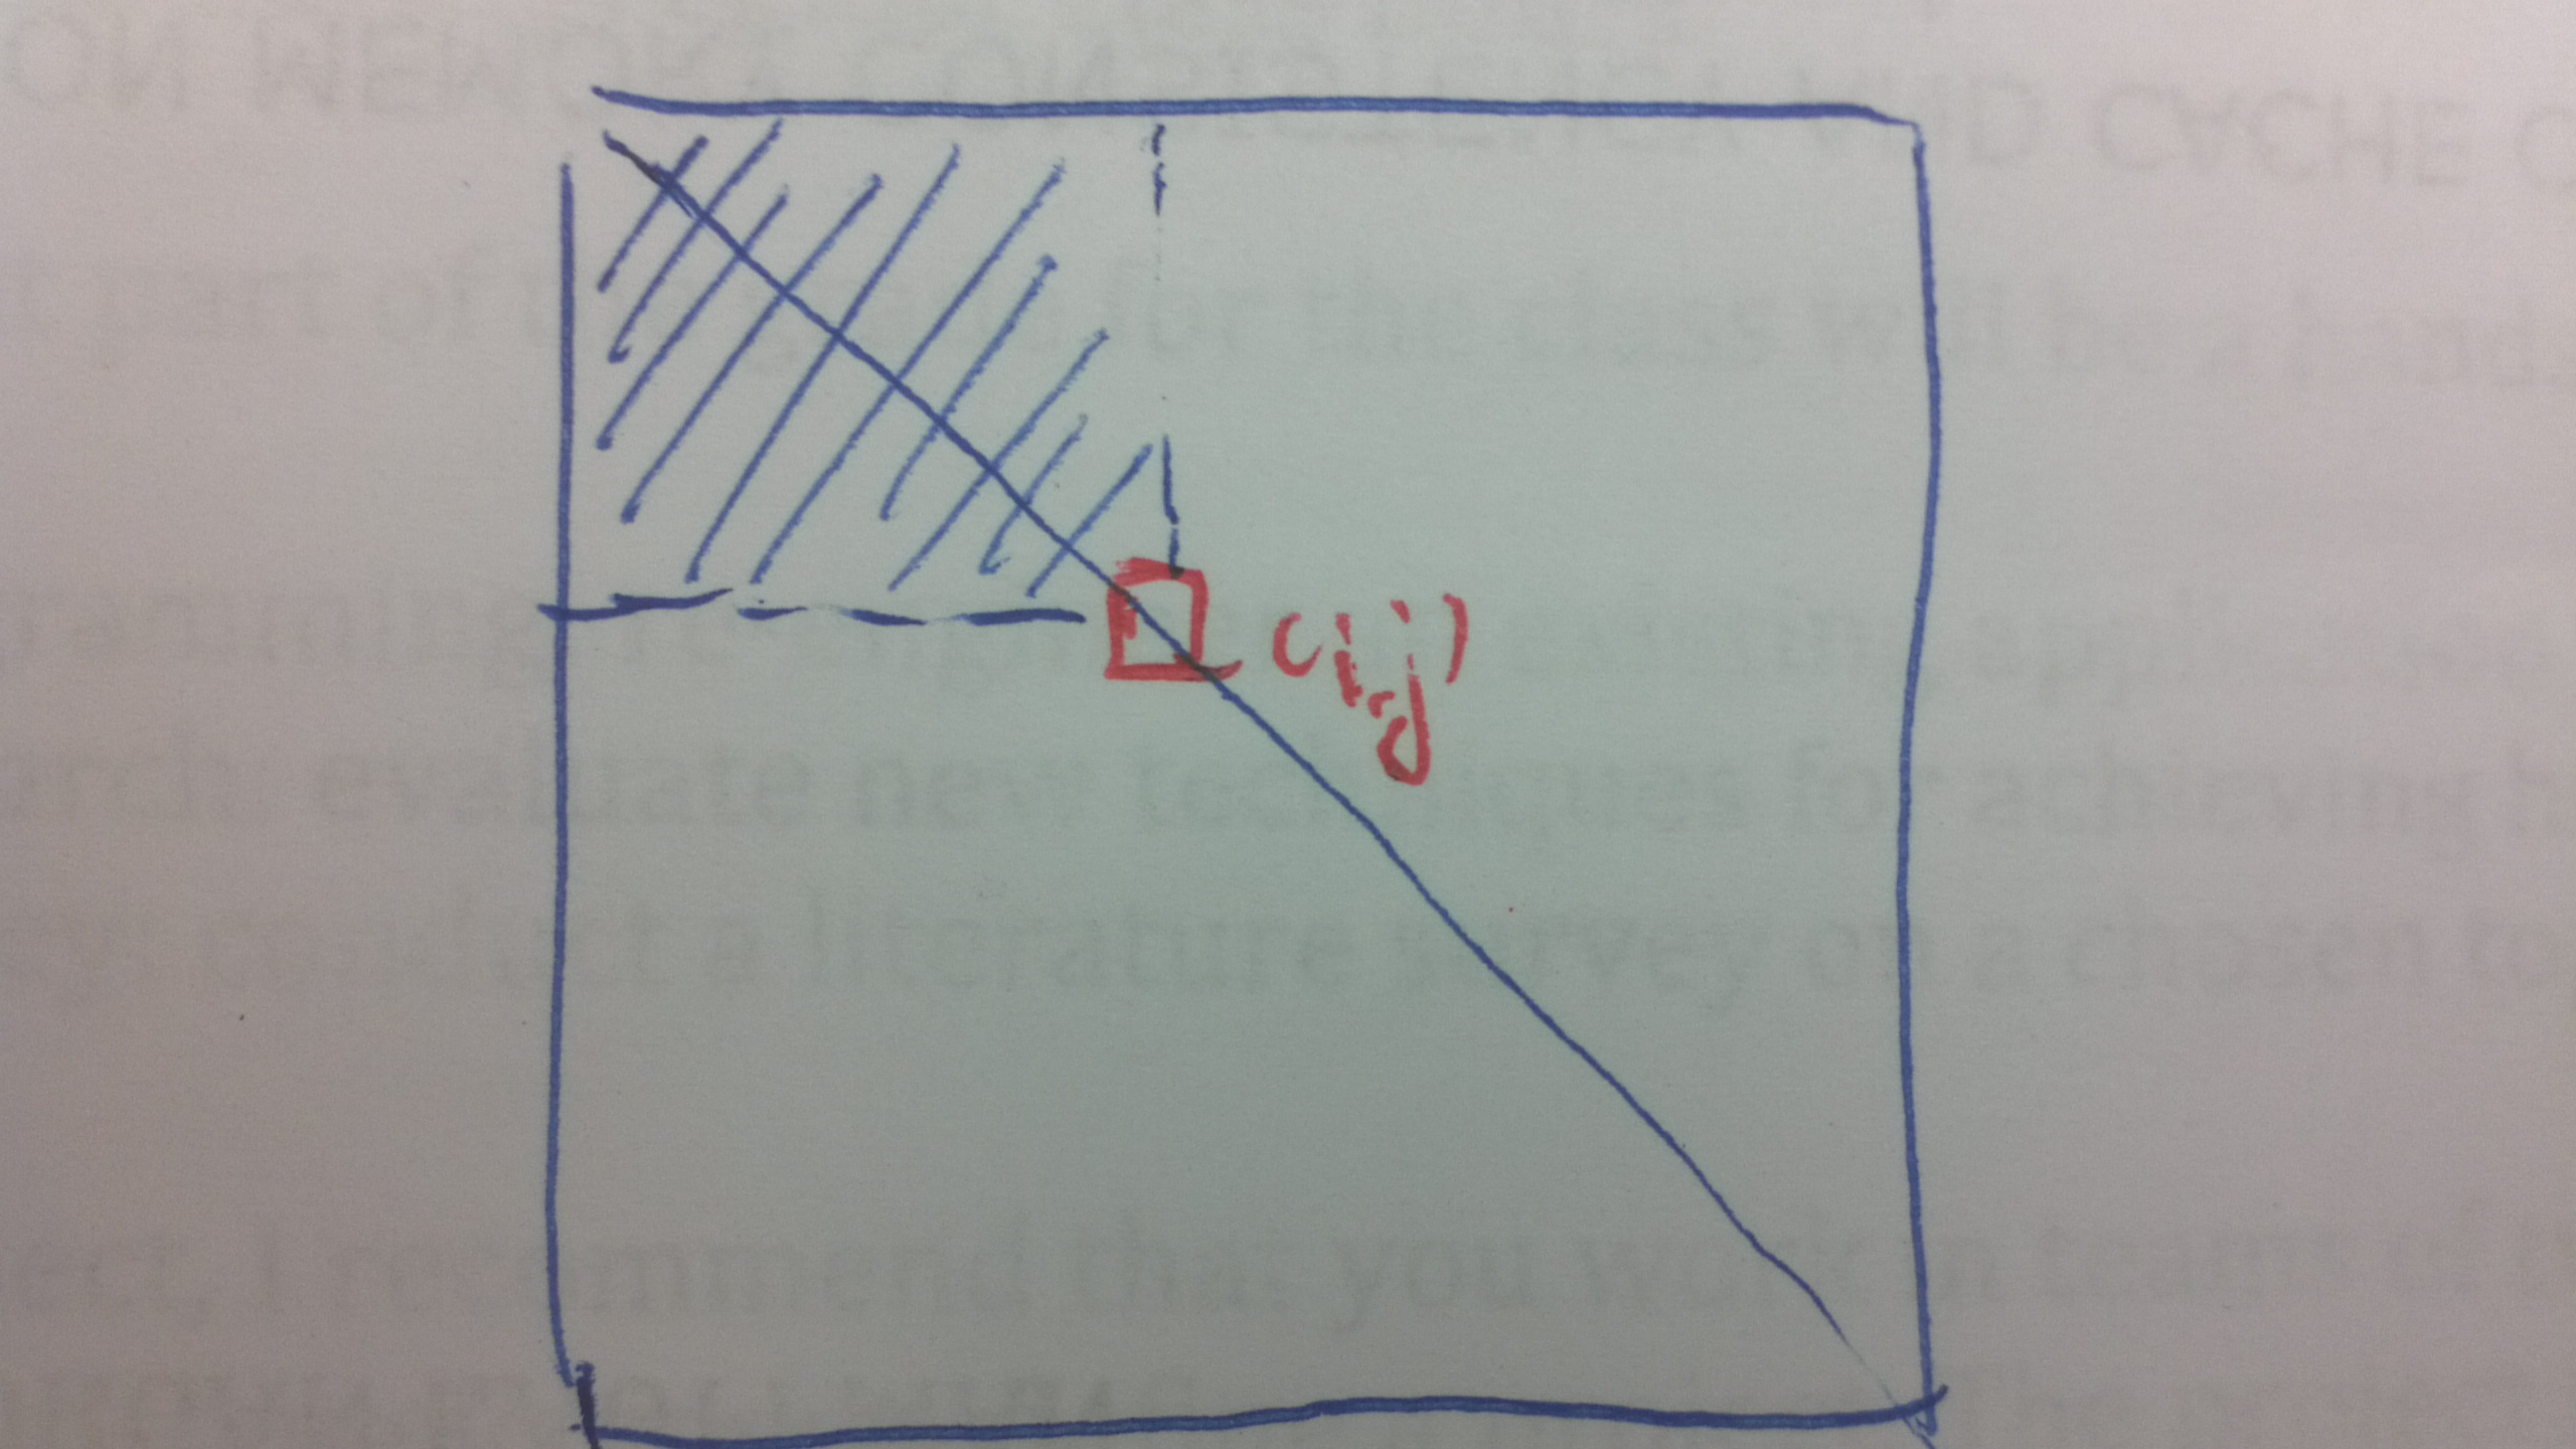
\includegraphics[width=\textwidth]{figures/a3.jpg}
\caption{dependences of entry $a_{i,j}$, where i = j}
\end{figure}

\subsection{2.7(b)}

%\lstinputlisting{src/b.cpp}
See src/b.cpp. 

\subsection{2.7(c)}

TODO: what's any form of async message passing?

Here's sync message passing program. (draft code, not compiled) 

%\lstinputlisting{src/c.cpp}
See src/c.cpp

\subsection{2.7(d)}

The only issue I see about the partitioning is that each pivot has different number of workload.
This imbalance could caue some threads/processes remaining idle. 

\subsection{2.7(e)}
I didn't see a reason why we want an interleaved version. 
There's no dependency between consecutive rows.

\subsection{2.7(f)} 
In this particular problem, I would prefer to use shared variable approach. 
\begin{enumerate}
\item It's much shorter, as I mentioned in the class.
\item Message passing version involves a huge data communication cost, 
\end{enumerate} 
especially in a network environment. 
Because in each iteration, we need to spread out almost the whole matrix. 
